\documentclass[UTF8]{article}
\usepackage[a4paper,bindingoffset=0.2in,%
            left=2cm,right=2cm,top=1in,bottom=1in,%
            ]{geometry}
\usepackage{ctex}
\usepackage{graphicx}
\usepackage{subfigure}
\usepackage{tcolorbox}
\tcbuselibrary{skins}
\usepackage{ulem}
\usepackage{float}
\usepackage{enumitem}
\usepackage{caption}
\usepackage{url}
\setlist{labelindent=\parindent}
\setlist[enumerate]{label=\textbf{\arabic*}}
\setlist{noitemsep,labelindent=\parindent}


\begin{document}

\begin{titlepage}
\title{\bfseries 移动互联网课程项目报告\\ --Let's Go: 基于位置的游玩分享软件}
\author{林士翰 15307130120, 赵浯旭 15307130231}
\date{}
\maketitle
\tableofcontents
\thispagestyle{empty}
\end{titlepage}

\section{项目概述}
Let's Go是一款能够让用户基于地理位置来记录和分享自己足迹的APP,它主要包含三大板块:留下足迹、探索、Go。
“留下足迹”可以根据当前的位置,选择附近的一个POI(Point of Interest),留下此刻用户的所感所想;
“探索”功能可以在地图上点击附近POI的图标(marker),浏览他人曾经在这里留下的“足迹”;
“Go”功能是基于用户的兴趣爱好和附近一定范围的POI的特征予以地点推荐,从而鼓励出行,发现有趣的、适合自己的地点。

Let's Go的客户端采用原生Android开发,服务器用Apache HTTP Server配合CGI(Common Gateway Interface)和MySQL搭建,
并部署在阿里云上(域名: shiftlin.top; IP地址: 139.196.123.150)。

项目github地址:\url{https://github.com/FDUZJ908/Let-s_Go}


\section{项目亮点}
\subsection{市场需求}
Let's Go是一个基于地理位置的状态分享平台,并且提供了地点推荐服务。目前市面上有许多状态分享软件,如大众点评、微信朋友圈、Swarm等。
大众点评关注用户的消费行为和分享,不是游玩分享平台,而微信朋友圈不关注地理位置信息,注重好友之间的分享。
Swarm是一款基于地理位置的社交软件,但关注签到行为,而不是想法的分享。此外,Swarm只能浏览好友的签到,无法浏览某一地点的其他人签到,也没有POI推荐功能。
还有一些游记软件,如面包旅行,关注的是用户的旅游行为。用户以游记的方式记录自己的行程,而不是在POI分享自己的想法。
此外,Let's Go没有好友的功能,因而并非传统的社交软件,达到了游玩推荐的目的。
因此,Let's Go正好弥补了市面上基于位置的游玩分享软件的缺失。

\subsection{产品亮点}
\begin{enumerate}
    \item “足迹”板块的地点热度可视化。在查看附近的POI时,服务器返回来的地点数据,以颜色不同的图标显示在地图上,其颜色的深浅和地点热度呈正相关,给用户提供了更好的体验。
    \item “足迹”中带有上传照片、点赞、反对功能。
    \item 在“Go”板块中推荐地点时,采用和“足迹”中类似的想法,将返回来的地点数据可视化地呈现在地图上,提升用户体验。
\end{enumerate}

\subsection{技术亮点}
\begin{enumerate}
    \item 充分考虑了网络安全性。如数据传输全部采用HTTPS;用户密码利用sha1哈希后存储;利用token进行用户身份验证和状态记录。
    \item 基于协同过滤算法进行地点推荐,并通过问卷调查解决冷启动问题(cold-start problem)。
    \item 通过优化,降低响应延迟,提高服务器负载能力。如调整了HTTP1.1的keep-alive属性,设置客户端缓存,一些影响不大的数据采用延迟更新,数据库建立索引等。
\end{enumerate}

\section{项目难点}
\subsection{客户端难点}
\begin{enumerate}
    \item 与后台的数据传输,由于有图片上传的功能,于是最终使用JSON格式数据与后台交互数据。
    \item 用户更新个人信息时候的标签处理。由于想达到用户能简单更新自己标签的效果,故需要使用一个选择器(picker)帮助完成功能实现。
    \item 在POI足迹列表中的图片缓存难点。因为根据POI的热度不同,其下的足迹数量也大不相同。在某些热度很高的POI下面,过多的用户图片将影响加载的速度,于是要对POI足迹中(ListView)的图片进行缓存,降低用户在图片加载上面的消耗。
    \item 地点热度的可视化问题。利用百度地图提供的API,根据后台返还的数据,将代表不同热度的marker打在地图上面。
\end{enumerate}

\subsection{服务器难点}
\subsubsection{获取POI数据}
百度地图API提供了获取附近POI的功能,但是需要输入关键字从而返回相关的POI,用户无法一次性获得附近所有POI,体验较差,
所以需要将百度地图API的上海的POI爬下来,建立自己的POI数据库。\\
我们选取了以下10个关键字,作为POI的分类:

\begin{tcolorbox}[colback=white]
\begin{center}
餐饮美食, 教育学校, 文化艺术, 旅游景点, 购物商场\\
休闲娱乐, 政府机关, 医疗卫生, 住宅小区, 生活服务
\end{center}
\end{tcolorbox}

由于每次只能获取少量的POI,于是将上海划分为许多小格子,对于每个小格分别发送上述10个关键字,获取相关POI。
此外,百度地图API是异步调用,无法直接进行循环,所以需要用回调函数递归实现循环。
最终获得了约27万的上海POI数据。

\subsubsection{推荐算法}
Let's Go利用基于物品的协同过滤算法(item-item collaborative filtering)进行地点推荐。
算法把不同用户对物品的评分当成物品的特征向量,利用向量计算物品之间的相似程度,从而预测用户对某个物品的评分,把评分高的物品推荐给用户。
然而,将协同过滤算法应用在Let's Go中需要解决三个问题:
\begin{enumerate}
    \item 如何定义评分? 如果将是否去过某个地点(0和1)当做评分,不够准确。
    \item 算法需要获得其他用户的发帖情况,计算量大,对服务器造成压力,延迟高。
    \item 如何解决冷启动问题(cold-start problem)? 用户或POI没有历史记录怎么办? 
\end{enumerate}

1和2的解决方法是利用标签(tags)。

每个用户注册后,需要选择符合自己的标签,Let’s Go提供了以下36种可选标签:

\begin{tcolorbox}[colback=white]
\begin{center}
70后,80后,90后,00后,12个星座\\
美食, 文化,艺术,旅游,时尚,游戏,运动,科技,动漫,教育\\
乐观,忧郁, 外向,安静,自信,急躁,耐心,机智,坦率,幽默
\end{center}
\end{tcolorbox}

设$tags_{i,j}$ 为带有第$j$个标签的在第$i$个POI发过贴的用户数。
对于第$i$个POI,
\[v_i=(tags_{i,1},tags_{i,2},  …  ,tags_{i,36}),\]
即可以认为是其特征向量,这样就不需要获得其他用户的发帖情况来计算特征向量,从而解决了第2个问题。

第$i$个POI和第$j$个POI之间的相似度用向量余弦来衡量。
\[C_{i,j}=cos(v_i,v_j)\]
由于余弦的性质,两个POI之间的相似度只跟其标签分布有关,跟标签绝对数量无关。

用户$u$对地点$j$的评分为
\[M_j=\frac{\sum_{p \in U}tags_{j,p}}{\sum_{k=1}^{36}tags_{j,k}}+1\]
加1是为了防止$M_j$为0。

同时,考虑到POI热度对推荐的影响,
\[P_i=log_2(1+\frac{sum_i}{max\{sum_j\}})+1,\]
加1是为了防止$log$的真数和$P_i$为0。

那么用户$u$对地点$i$的评分为
\[Scores_i=max\{C_{i,j} \times M_j\} \times P_i\]

选出Scores最大的前$k$个POI推荐给用户,并保证每个分类都有POI被选取。

当POI没有历史记录时,就无法获得POI的特征向量,为此,我们进行了问卷调查。
问卷样式如下图,共5个问题,前4个问题为选择标签,第5个问题为选择感兴趣POI类别。
\begin{figure}[H]
\begin{minipage}[t]{0.15\textwidth}
    \vspace{0pt}
    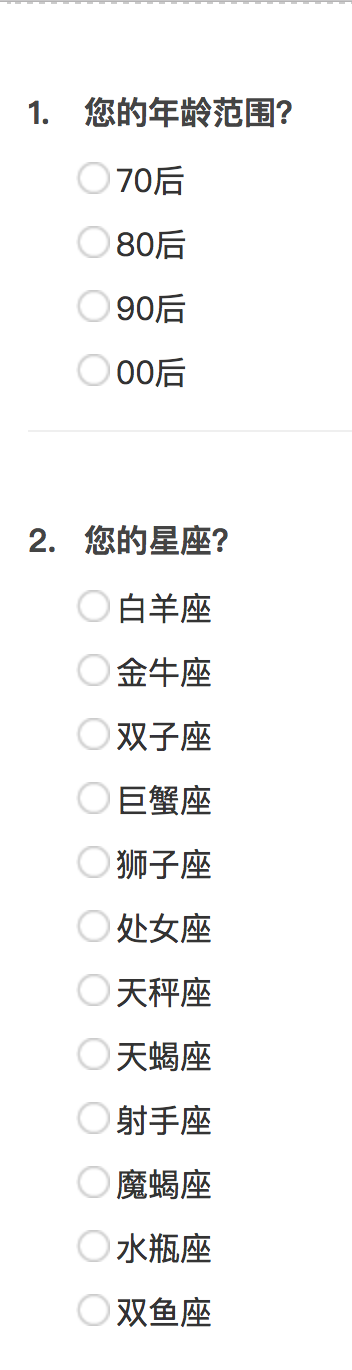
\includegraphics[width=\textwidth]{images/ques1.png}
\end{minipage}
\begin{minipage}[t]{0.45\textwidth}
    \vspace{0pt}
    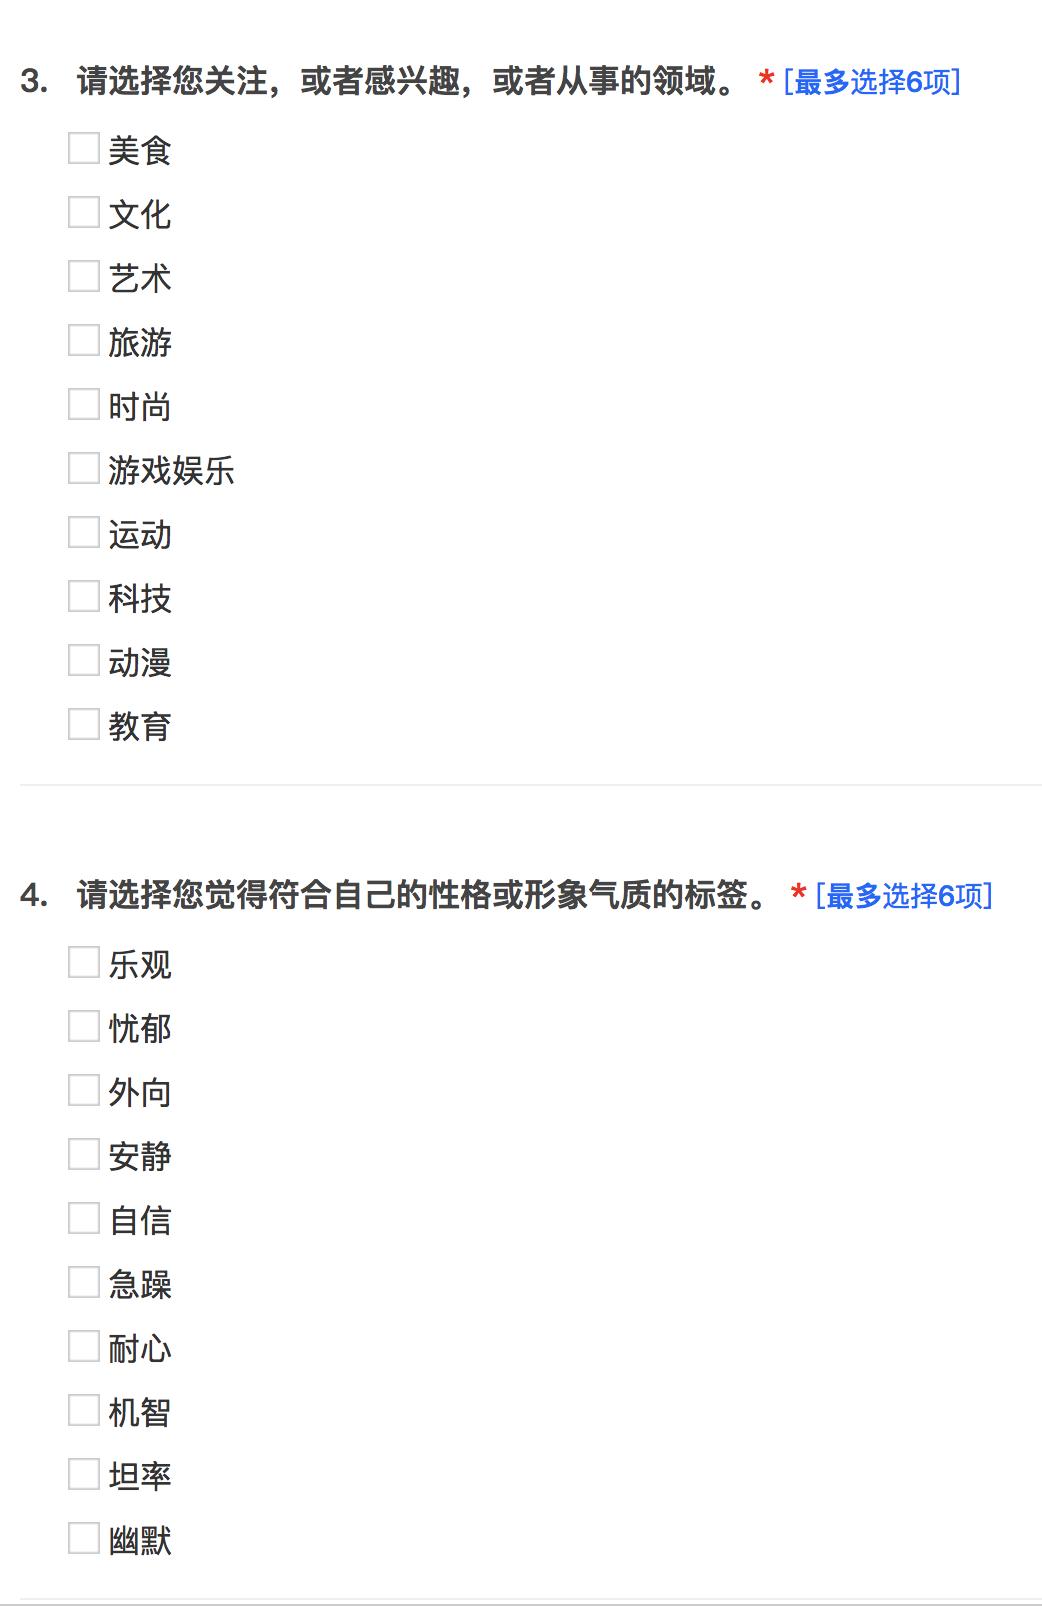
\includegraphics[width=\textwidth]{images/ques2.png}
\end{minipage}
\begin{minipage}[t]{0.4\textwidth}
    \vspace{0pt}
    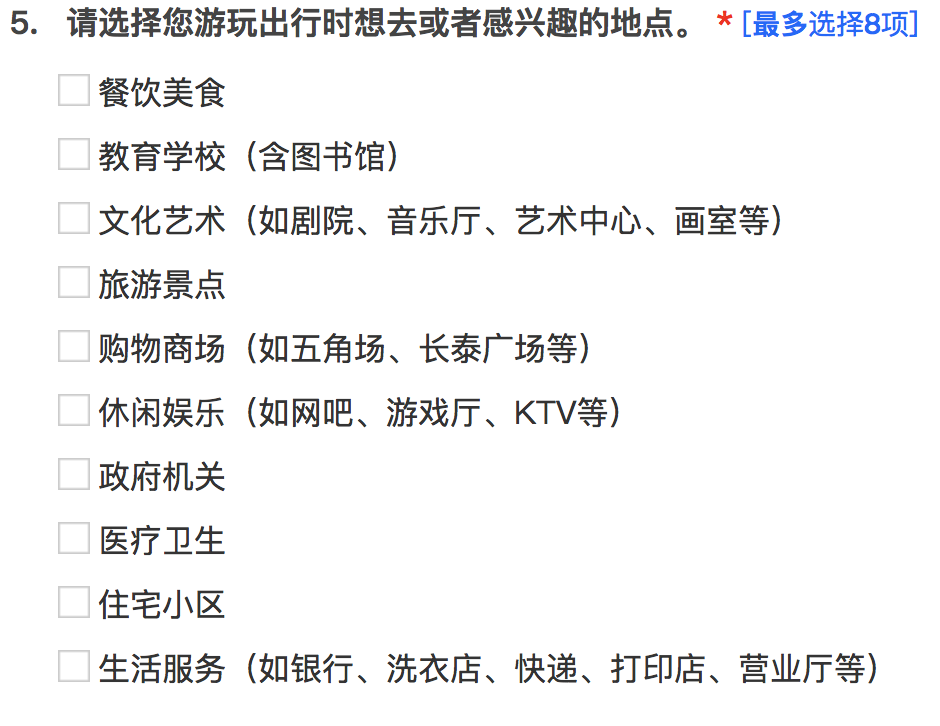
\includegraphics[width=\textwidth]{images/ques3.png}
\end{minipage}
\caption*{问卷地址: \url{https://www.wjx.cn/jq/19541006.aspx}}
\end{figure}
我们总共收集了146份调查问卷,这样就获得了每个POI类别的标签分布,将POI类别的标签分布作为POI的初始标签分布。
当POI没有历史记录时,其特征向量为其所属类别的特征向量;当POI有历史记录后,在初始向量上加上历史发帖用户的标签,得到特征向量。\\
当用户没有历史记录时,我们只考虑用户标签与POI特征向量匹配程度和POI热度的影响,$Scores_i$修正为$Scores_i=M_i \times P_i$。

\subsubsection{后端优化}
用户每一次发帖都会导致POI的标签改变,也会导致POI的热度(即该POI的帖子数)改变,同时,由于Apache CGI是运行在不同进程中,无法在内存里维护这些变化,给数据库增加很大的压力。考虑到POI的标签和热度只会影响推荐算法,单次发帖对推荐算法的影响很小,可以延迟更新。所以采用按天更新的机制,在服务器上设置定时器,每天凌晨3点的将前一天的所有发帖统计后写入数据库。

同样的,点赞和反对的请求比较频繁,对服务器也造成相当大压力,而且实时性要求较高,无法延迟更新。对于一次浏览某个POI的历史帖子(从点击POI的图标到点击返回键),客户端将用户的点赞反对行为积攒下来,当用户退出浏览后再一起发送给服务器,服务器写入数据库,从而减小服务器压力。

客户端对用户位置和POI进行缓存,当用户位置变化不大时,就不需要再次向服务器查询附近的POI和推荐地点,直接返回上一次结果。

发帖和推荐都需要获得用户的标签,如果直接从数据库获取会增加数据库访问次数,改为由客户端提供。当用户发帖或者需要推荐时,客户端就将用户的标签发给服务器,服务器就不需要从数据库获得用户的标签,减少了数据库访问次数。只有当用户在个人信息页面获取或修改标签时,服务器才会访问数据库的标签数据。此外,由于标签数有36个,为了减少网络传输流量,将标签进行比特编码,第$i$位为1表示有$i$号标签,第$i$位为0表示没有$i$号标签,这样只要一个64位整数就可以表示用户的标签了。

对于客户端的所有请求,服务器都需要验证用户的身份。对于session机制,用户登录时服务器分配一个sessionid给客户端,客户端的所有请求都需要附上ssesionid,由于CGI在不同进程的原因,服务器需要访问数据库进行检验,这给数据库增加了很大压力。

因此,我们采用了token机制。用户登录时服务器返回一个token给客户端。token由两部分组成,一个是由用户ID和一个随机数连接而成的字符串$S$,另一个是对字符串$S$进行哈希后得到的字符$H$,token由$S$和$H$连接而成。
这样,客户端的所有请求都附上token,服务器提取出token的字符串$S$,以同样的方式进行哈希,得到$H'$,比对$H$和$H'$,如果相等则检验通过。
这样就完全不需要进行数据库访问,只要计算哈希值即可。字符串$S$中的随机数是为了使得同一用户每次产生的token不固定。

这里的哈希算法采用如下方式:先对$S$进行多项式哈希,底数在服务器启动时决定,此后保持不变,不能泄漏;然后再进行sha1哈希,得到$H$。采用两层哈希的原因是,sha1没有密钥输入,token容易被伪造,所以将多项式哈希的底数和哈希方式作为服务器密钥输入给该哈希算法。

\section{源代码说明}
\subsection{技术清单}
客户端:
\begin{enumerate}
    \item Android原生Activity、Fragment组件,ListView、ImageView控件
    \item SharedPreferences用于存储用户账号密码等数据
    \item 百度地图提供的BaiduLBS API
    \item okhttp3用户与后台网络传输数据
    \item Gson用于转换Java对象和JSON对象
    \item android-pickers用于实现选择器操作
    \item LabelsView用于实现标签选择
    \item universal-image-loader用于实现加载、缓存图片
    \item picasso用于实现图片异步下载
\end{enumerate}

服务器:
\begin{enumerate}
    \item Apache HTTP Server和CGI用于基本服务器框架搭建
    \item 阿里云域名注册和解析,HTTPS证书申请和配置
    \item linux C++开发工具链(g++, make, shell脚本)
    \item C++ rapidjson库用于解析JSON
    \item MySQL Connector C++和MySQL Connector Python分别用于C++和Python访问数据库
    \item openssl用于实现sha1哈希
    \item Python利用SMTP实现发送验证码到用户邮箱
    \item 服务器用crontab实现定时任务
\end{enumerate}

\subsection{目录结构及代码重要模块介绍}
客户端:
\begin{figure}[H]
    \center
    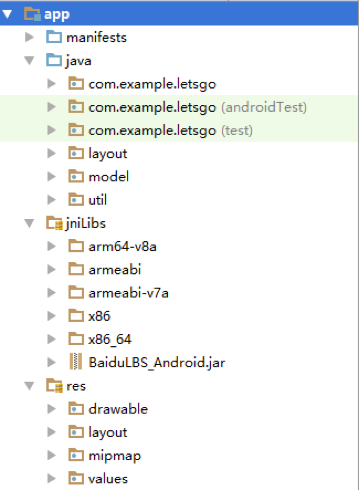
\includegraphics[width=0.3\textwidth]{images/client1.png}
\end{figure}
\begin{enumerate}
    \item letsgo目录下方为主要的Activity,其中DataActivity为爬取百度地图数据的时候用到,在APP中是无效的。按照其命名,可以得到它们各自代表的含义。其中在MainActivity中完成了程序启动后的初始化,包括处理3个fragment、设置权限、判断是否有登录缓存等。
    \begin{figure}[H]
    \center
    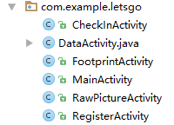
\includegraphics[width=0.3\textwidth]{images/client2.png}
    \end{figure}

    \item layout目录下存在4个Fragment,其中Fragment1代表未登录时的界面,Fragment2、Fragment3、Fragment4分别代表“足迹”模块、“Go”模块、“个人”模块。
    \begin{figure}[H]
    \center
    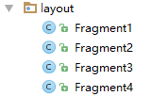
\includegraphics[width=0.3\textwidth]{images/client3.png}
    \end{figure}

    \item model目录下为相关类定义。其中FootprintAdapter是足迹ListView的适配器,其中包括了对文字、图片的处理,点赞、反对机制的处理等。
    \begin{figure}[H]
    \center
    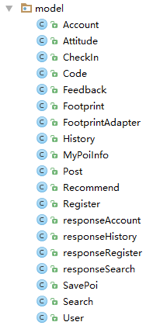
\includegraphics[width=0.3\textwidth]{images/client4.png}
    \end{figure}

    \item util目录下定义相关工具。Check包含判断是否为正确的电话、邮箱格式;Convert包含数据之间的相关转换;httpUtil包含通过okhttp发送Get, Post请求;ImageUtils包含对图片的压缩和向String转换的功能;Picker主要是定义选择年龄、性别、星座的选择器。
    \begin{figure}[H]
    \center
    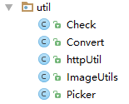
\includegraphics[width=0.2\textwidth]{images/client5.png}
    \end{figure}

    \item jniLibs目录下包括百度LBS提供的相关接口,在后面的环境配置中会详述。
    \begin{figure}[H]
    \center
    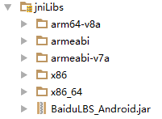
\includegraphics[width=0.3\textwidth]{images/client6.png}
    \end{figure}

    \item res目录下包括前端UI的布局相关文件。涵盖布局文件、图片等。
    \begin{figure}[H]
    \center
    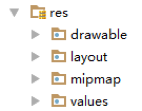
\includegraphics[width=0.2\textwidth]{images/client7.png}
    \end{figure}
\end{enumerate}

服务器:
\begin{figure}[H]
    \center
    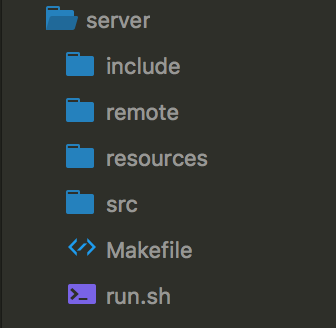
\includegraphics[width=0.3\textwidth]{images/server1.png}
\end{figure}
\begin{enumerate}
    \item src目录下为CGI的源代码和数据库的SQL语句,以及一些辅助功能的代码。\\
    \begin{figure}[H]
    \center
    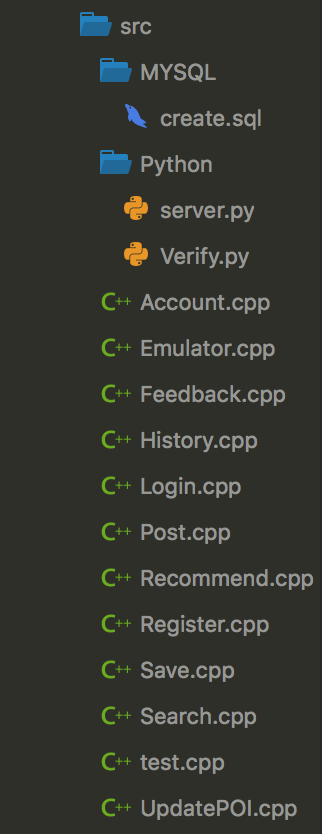
\includegraphics[width=0.2\textwidth]{images/server3.png}
    \end{figure}
    \begin{tcolorbox}[colback=white]
        Python/server.py, Python/Verify.py: 采用SMTP协议发送验证码到客户邮箱。\\
        Account.cpp: 获取帐号信息或更新个人信息。\\
        Emulator.cpp: 生成随机数据做示例。\\
        Feedback.cpp: 点赞/反对功能。\\
        History.cpp: 获取某一地点的历史发帖。\\
        Post.cpp: 处理用户发帖请求。\\
        Recommend.cpp: 推荐算法。\\
        Register.cpp: 用户注册。\\
        Save.cpp: 保存爬虫的结果。\\
        Search.cpp: 获取附近的POI。\\
        test.cpp: 测试代码。\\
        UpdatePOI.cpp: 更新POI的标签和热度,每天由crontab运行一次。
    \end{tcolorbox}

    \item include目录下为一些头文件,对底层库进行了封装。\\
    \begin{figure}[H]
    \center
    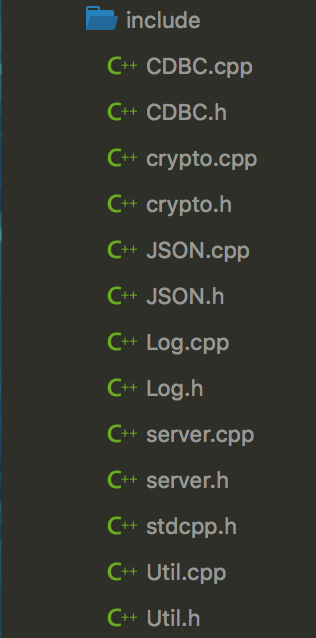
\includegraphics[width=0.2\textwidth]{images/server2.png}
    \end{figure}
    \begin{tcolorbox}[colback=white]
        CDBC.h, CDBC.cpp: 对mysql-connector-c++进行封装。\\
        crypto.h, crypto.cpp: 哈希函数和Base64解码。\\
        JSON.h, JSON.cpp: 对rapidjson进行封装。\\
        Log.h, Log.cpp: 打印日志。\\
        server.h, server.cpp: \\
        Util.h, Util.cpp: 一些辅助工具,如类型转换,时间转换等。
    \end{tcolorbox}

    \item remote目录下为放置在服务器上的辅助脚本。\\
    \begin{figure}[H]
    \center
    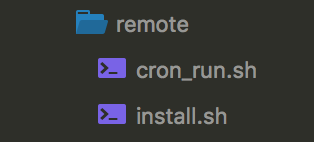
\includegraphics[width=0.3\textwidth]{images/server4.png}
    \end{figure}
    \begin{tcolorbox}[colback=white]
        cron\_run.sh: crontab定时任务。\\
        install.sh: 本地执行make install命令时,服务器上执行这一脚本来编译并部署CGI。
    \end{tcolorbox}

    \item resources目录下只有category.txt,为问卷调查的结果。
    \begin{figure}[H]
    \center
    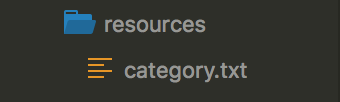
\includegraphics[width=0.3\textwidth]{images/server5.png}
    \end{figure}

    \item Makefile为make文件,用于编译控制。
    \item run.sh用于初始化环境(--conf选项)和调试时辅助运行指定CGI。
\end{enumerate}

\subsection{环境配置、编译、安装指南}
\subsubsection{客户端}
客户端可以直接使用提供的app-release.apk安装,也可以编译源码运行,在Android Studio中编译源码并运行的步骤如下:
\begin{enumerate}
    \item 将/LetsGo文件夹导入Android Studio中。
    \item 在\url{http://lbsyun.baidu.com/index.php?title=sdk/download\&action}下载百度地图SDK(请按下图选择)。
    \begin{figure}[H]
    \center
    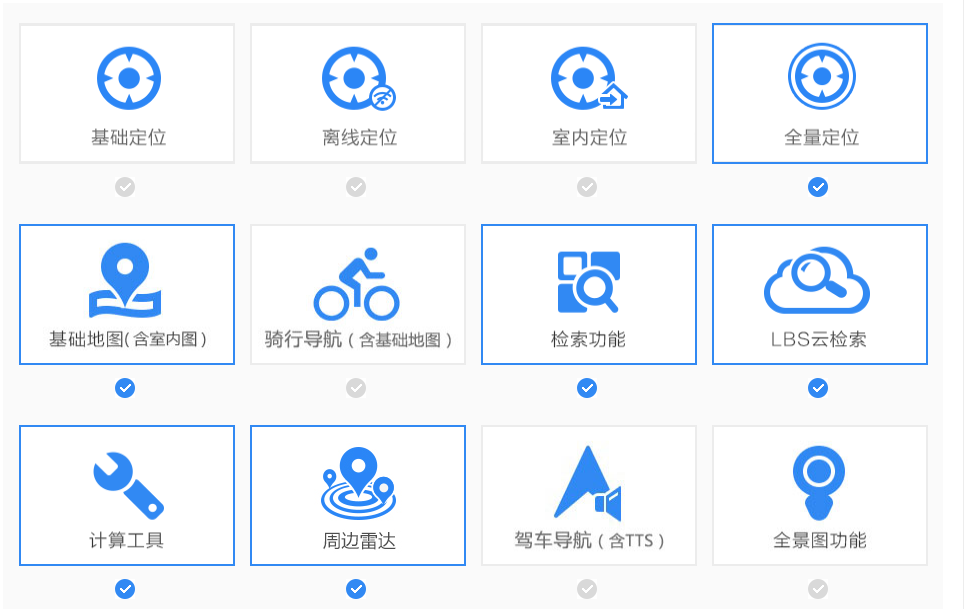
\includegraphics[width=\textwidth]{images/baiduAPI.png}
    \end{figure}
    \item 解压BaiduLBS\_AndroidSDK\_Lib.zip得到libs文件夹,其中包含BaiduLBS\_Android.jar以及其他5个文件夹(arm64-v8a,armeabi,armeabi-v7a,x86,x86\_64)。
    \item 在/LetsGo/app下新建libs文件夹,将上述BaiduLBS\_Android.jar拷贝至/LetsGo/app/libs目录下。
    \item 在/LetsGo/app/src/main下新建jniLibs文件夹,将上述5个文件夹拷贝至/LetsGo/app/src/main/jniLibs目录下。
    \item 更改/LetsGo/gradle/wrapper/gradle-wrapper.properties中的gradle-2.x-all.zip为gradle-3.3-all.zip。
    \item 编译,使用AVD或真机即可运行。
\end{enumerate}

\subsubsection{服务器}
由于操作系统和依赖包安装方式等千差万别,服务器的搭建步骤不唯一,但本质是一样的。客户端使用的是已经部署好的阿里云服务器(域名: shiftlin.top; IP地址: 139.196.123.150)。这里以该服务器(Centos 7)为例,简略叙述搭建步骤。
\begin{enumerate}
    \item 在服务器上安装Apache, mysql, rapidjson, openssl, mysql-connector-c++, mysql-connector-python。
    \item 编辑/etc/httpd/conf/httpd.conf,配置Apache,需要配置HTTPS。
    \item 将/server目录拷贝到服务器上/root目录下,并且重命名为LetsGo。
    \item 在LetsGo目录下,执行命令bash ./run.sh - -conf,然后执行命令make编译。
    \item 编译成功后将LetsGo/cgi-bin目录下的可执行文件和LetsGo/src/Python目录下的脚本全部复制到/var/www/cgi-bin目录中。
    \item 根据LetsGo/src/MYSQL/create.sql文件,建立好数据库,导入POI数据。
    \item 在/root/.bash\_profile和/etc/httpd/conf/httpd.conf中都添加以下环境变量。\\
    \begin{tcolorbox}[colback=white]
        DatabasePassword ``1234" //数据库密码\\
        EmailAddress ``test@163.com" //用来发验证码的邮箱\\
        EmailPassword ``123456" //邮箱密码\\
        HASHSEED ``960821" //多项式哈希种子\\
        \\
        LetsGoLogPATH ``/root/Log/" \\
        //日志文件存储目录,需要先手动建立,并且设置权限为777\\
        LetsGoResrcPATH ``/root/LetsGo/resources/"\\
        //资源文件目录,需要设置权限为777\\
        LetsGoFilePATH ``/var/www/html/Files/" \\
        //用户上传的图片保存目录,需要手动建立,并且设置权限为777
    \end{tcolorbox}
    \item 配置linux的crontab定时任务,使其定时运行LetsGo/remote/下的cron\_run.sh。
    \item 用命令service httpd start运行Apache。
\end{enumerate}

\section{APP重要使用场景}
\begin{figure}[H]
\begin{minipage}[t]{0.33\textwidth}
    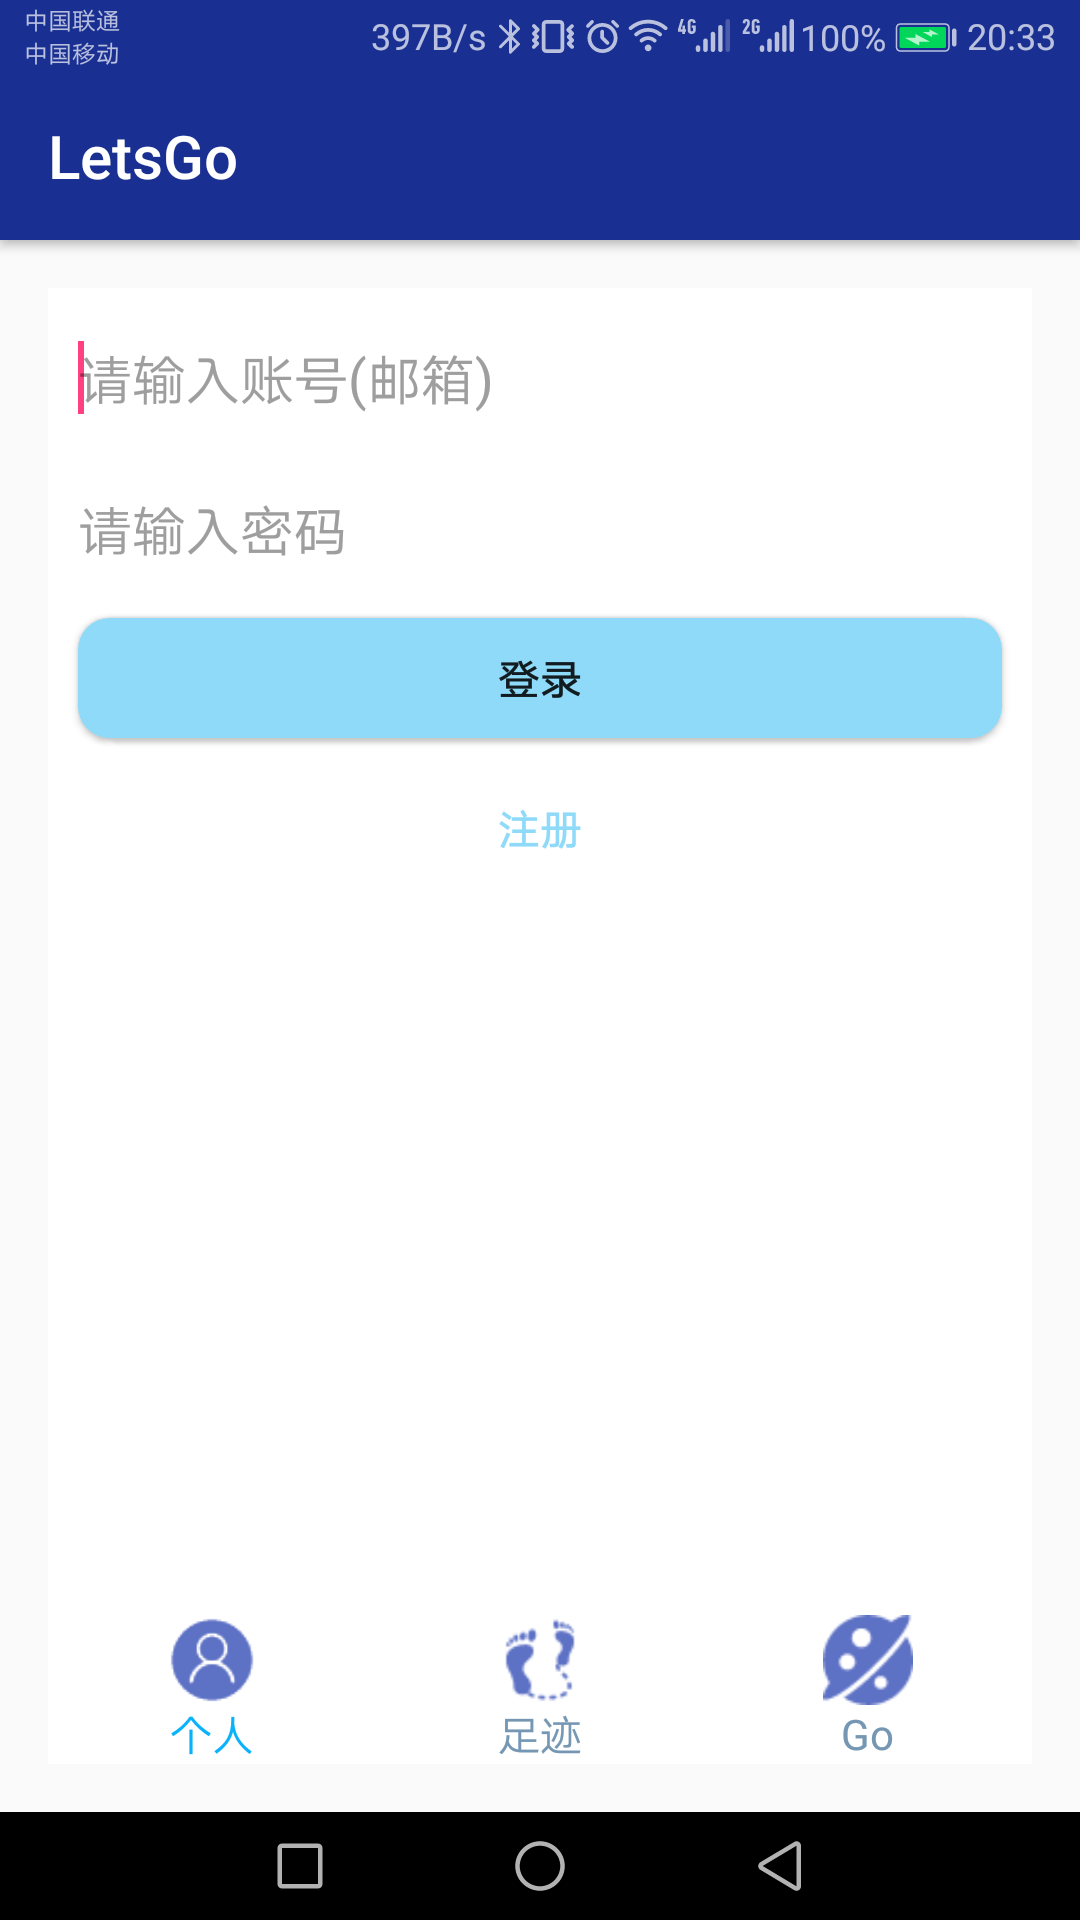
\includegraphics[width=\textwidth]{images/demo_login.png}
    \caption{登录}
\end{minipage}
\begin{minipage}[t]{0.33\textwidth}
    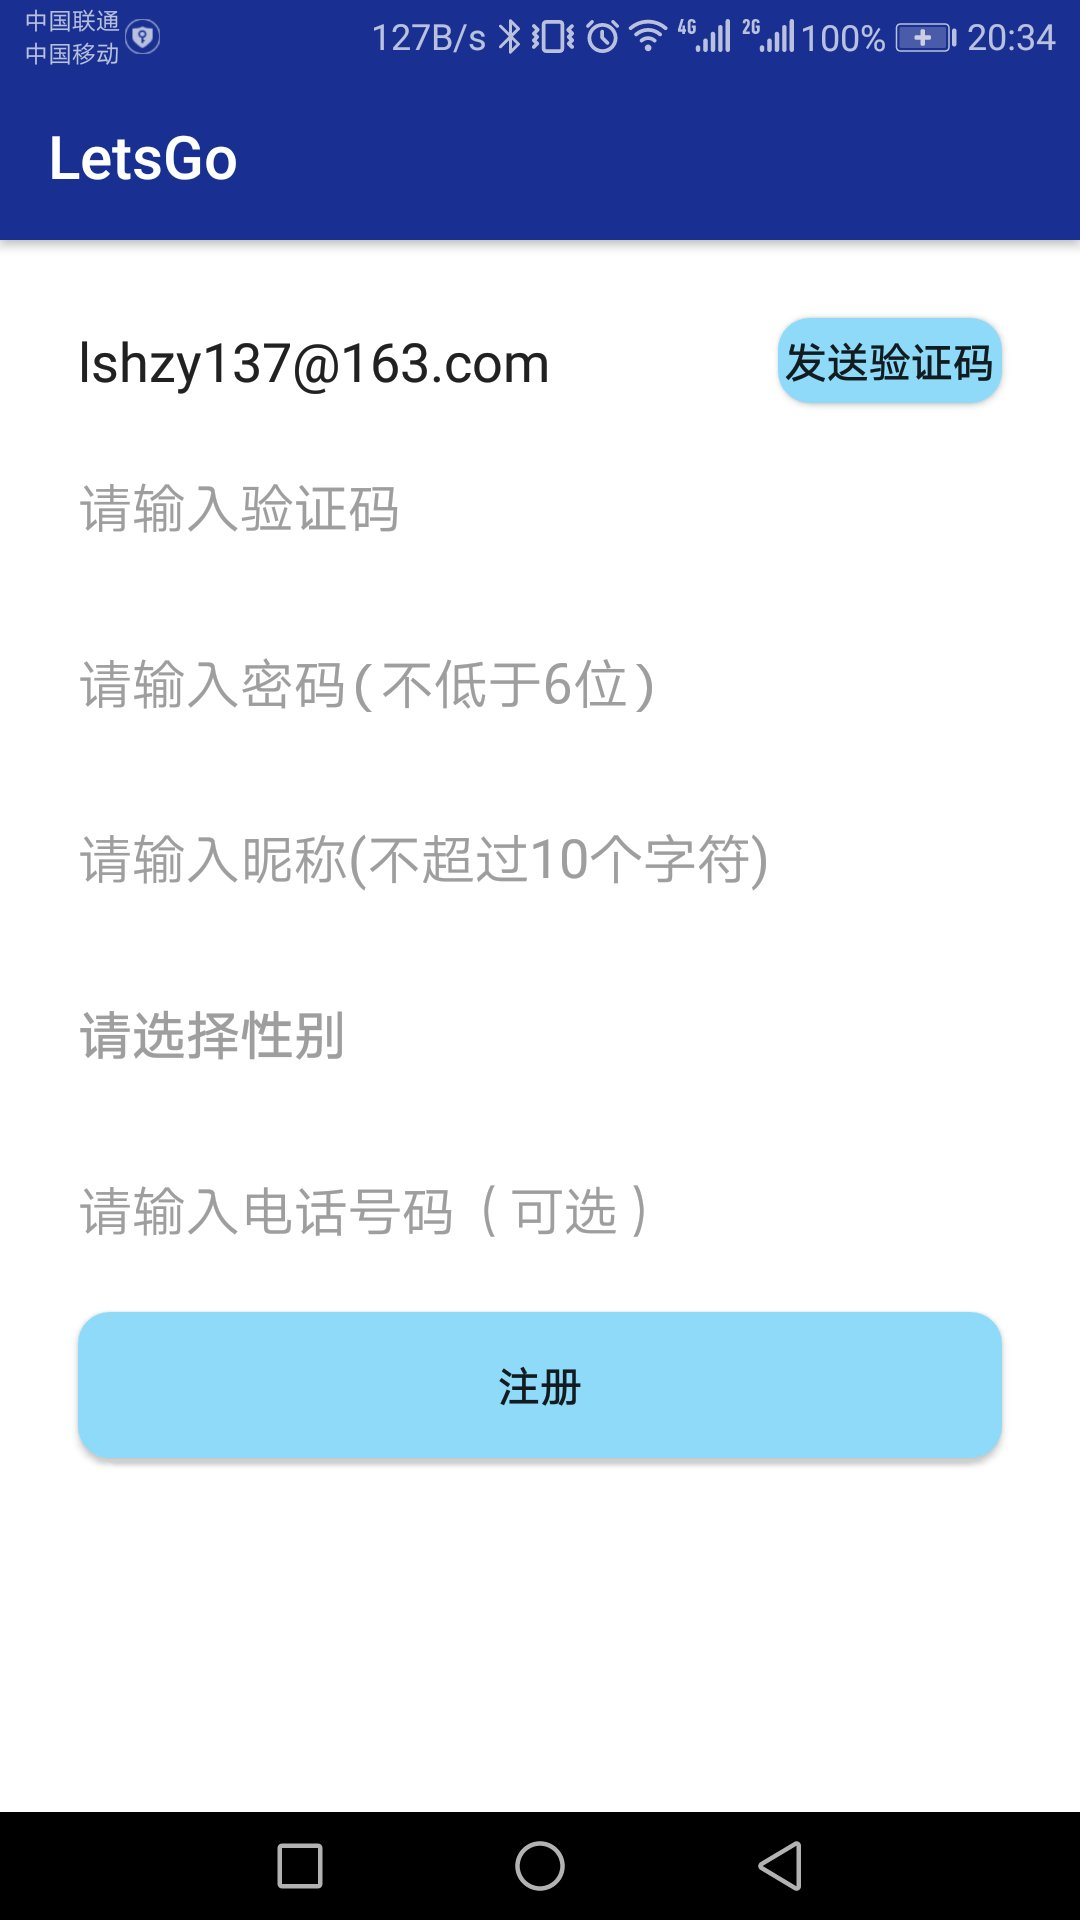
\includegraphics[width=\textwidth]{images/demo_register.jpeg}
    \caption{注册}
\end{minipage}
\begin{minipage}[t]{0.33\textwidth}
    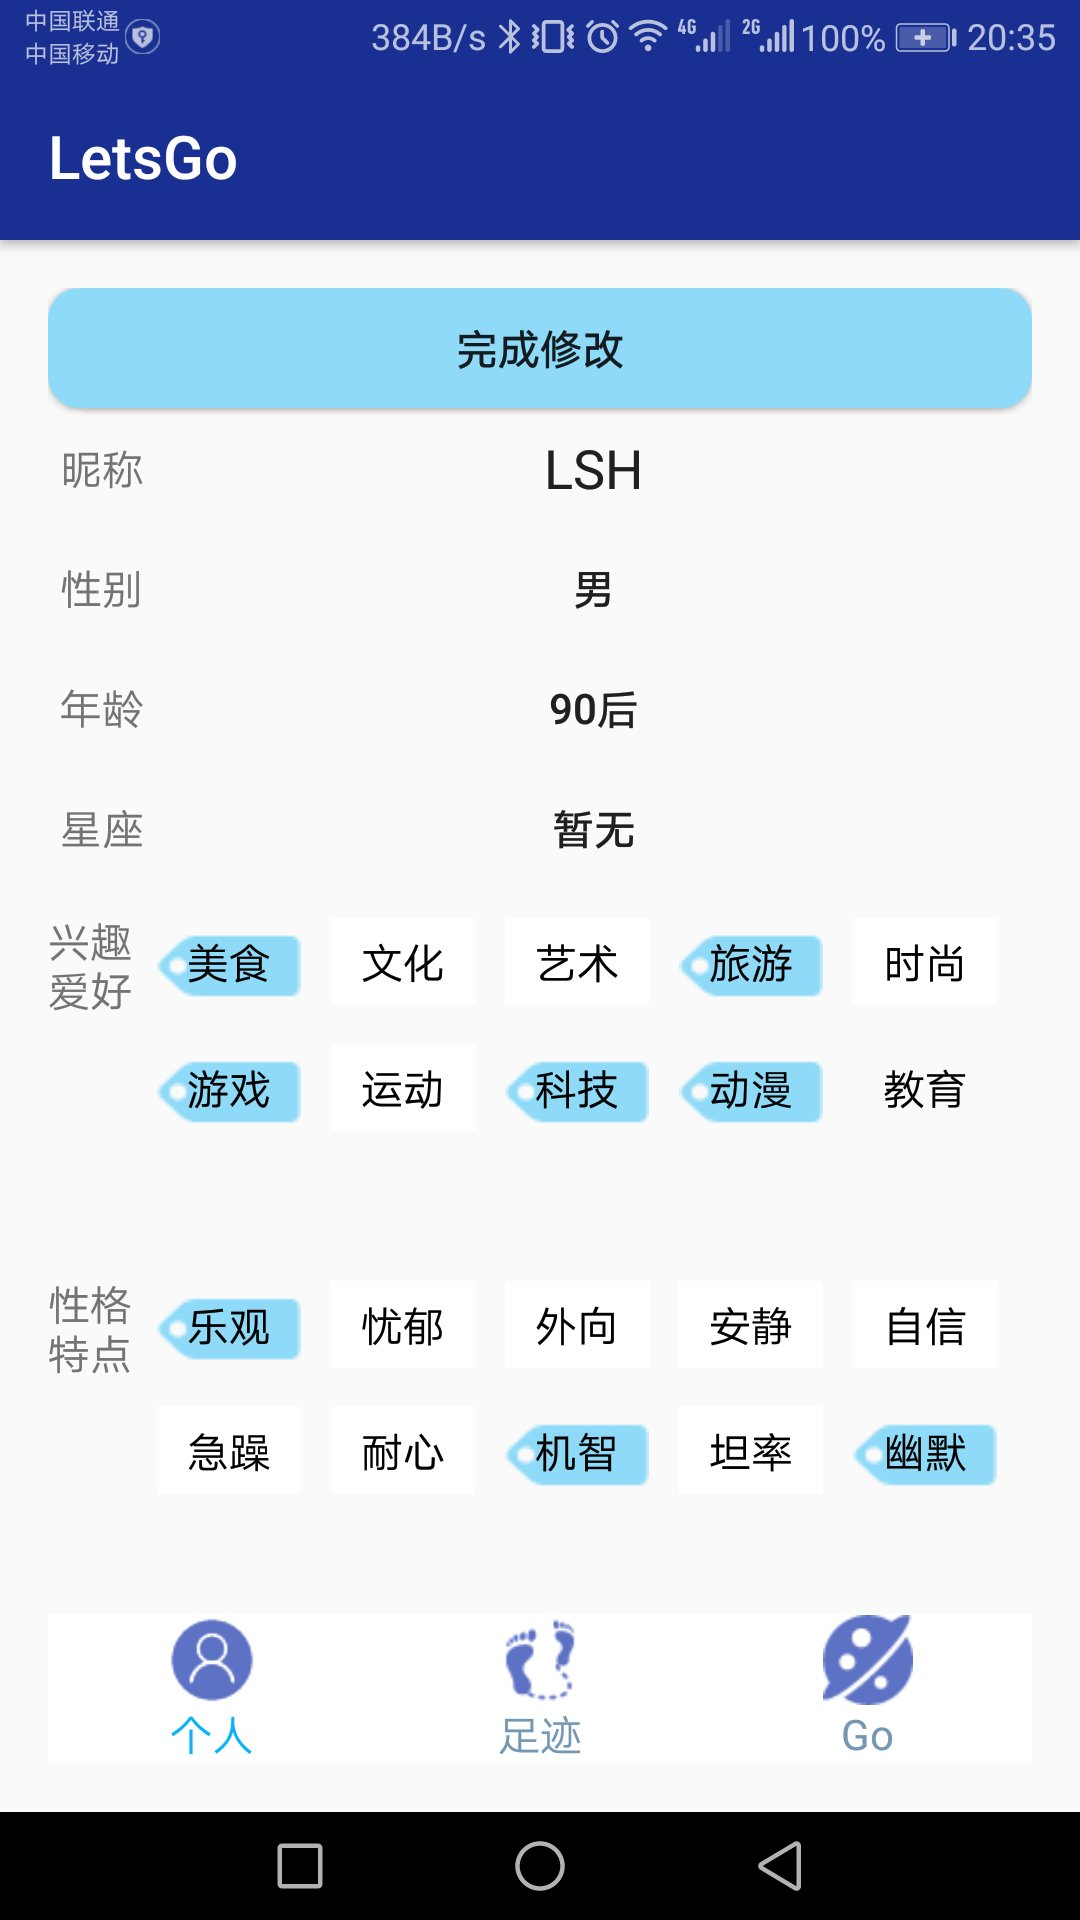
\includegraphics[width=\textwidth]{images/demo_profile.jpeg}
    \caption{查看和修改个人信息}
\end{minipage}
\end{figure}

\begin{figure}[H]
\begin{minipage}[t]{0.33\textwidth}
    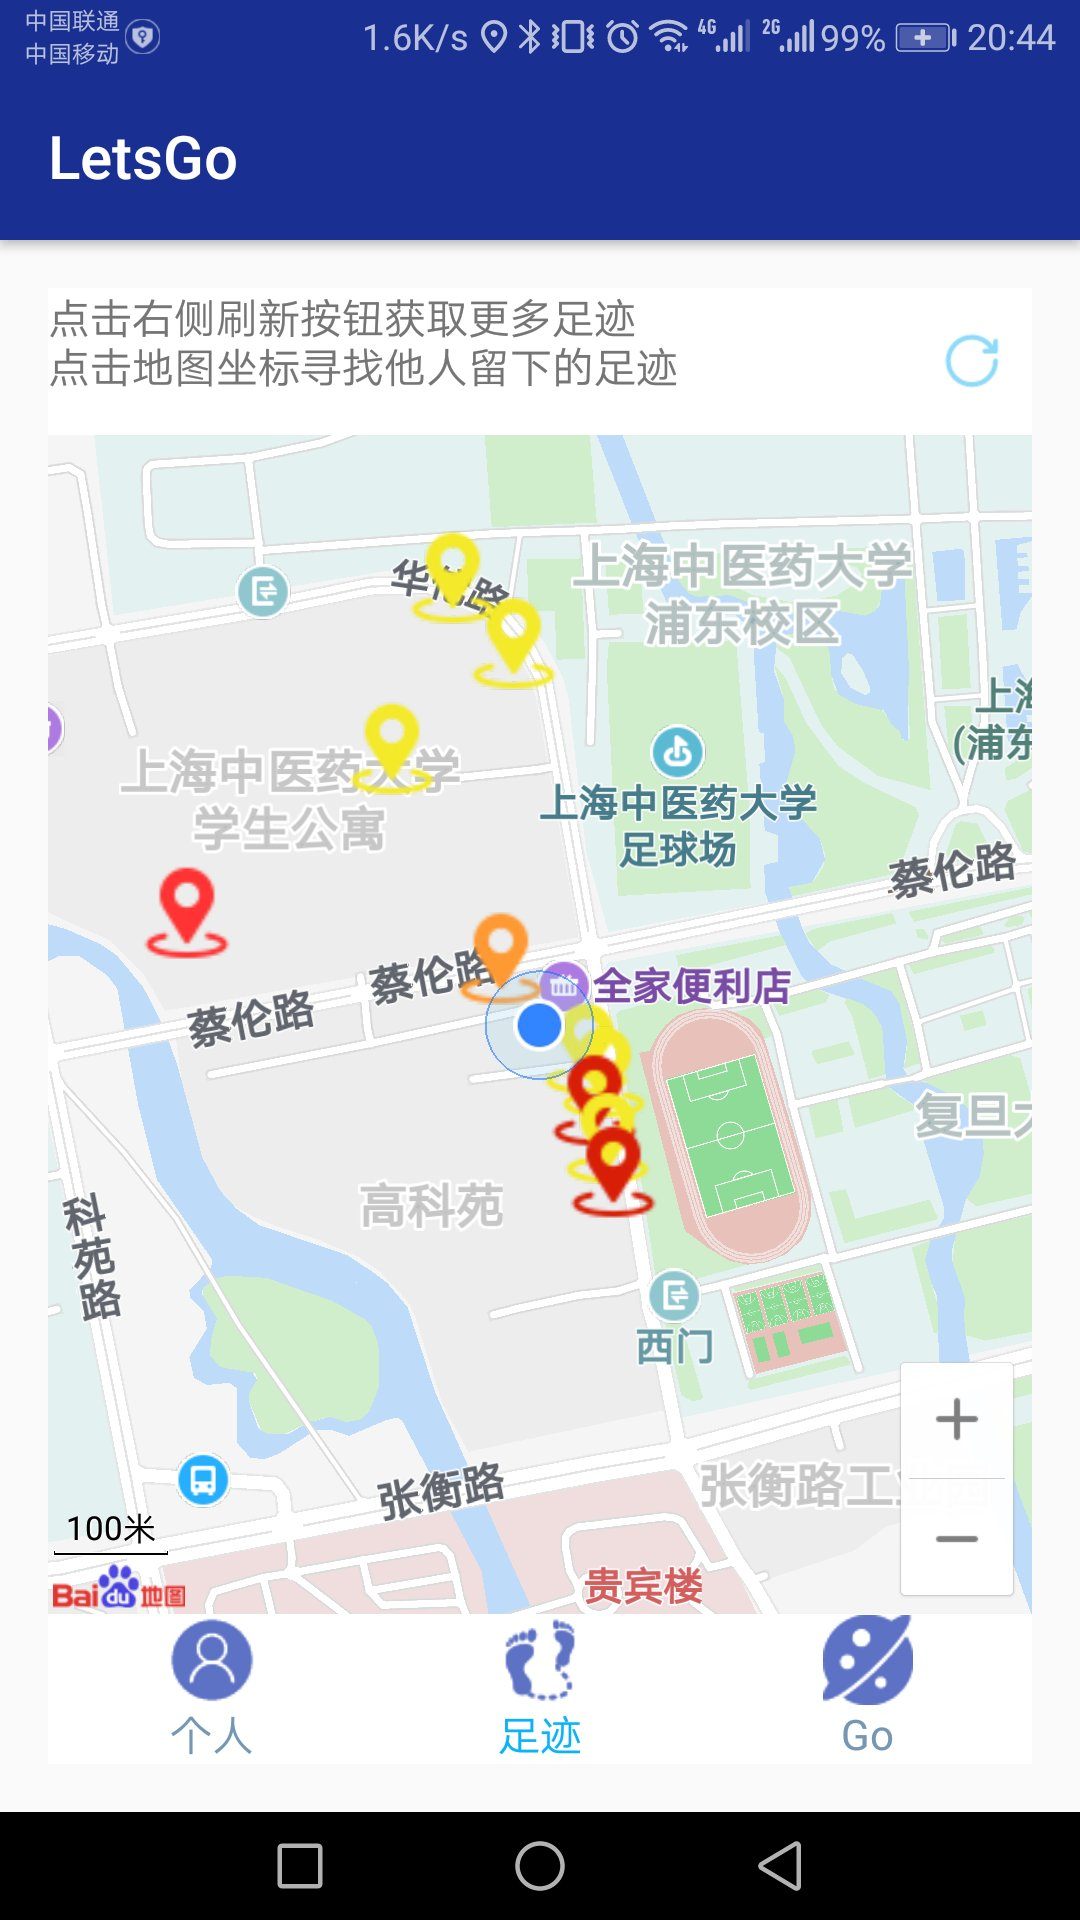
\includegraphics[width=\textwidth]{images/demo_POI.jpeg}
    \caption{查看附近的POI}
\end{minipage}
\begin{minipage}[t]{0.33\textwidth}
    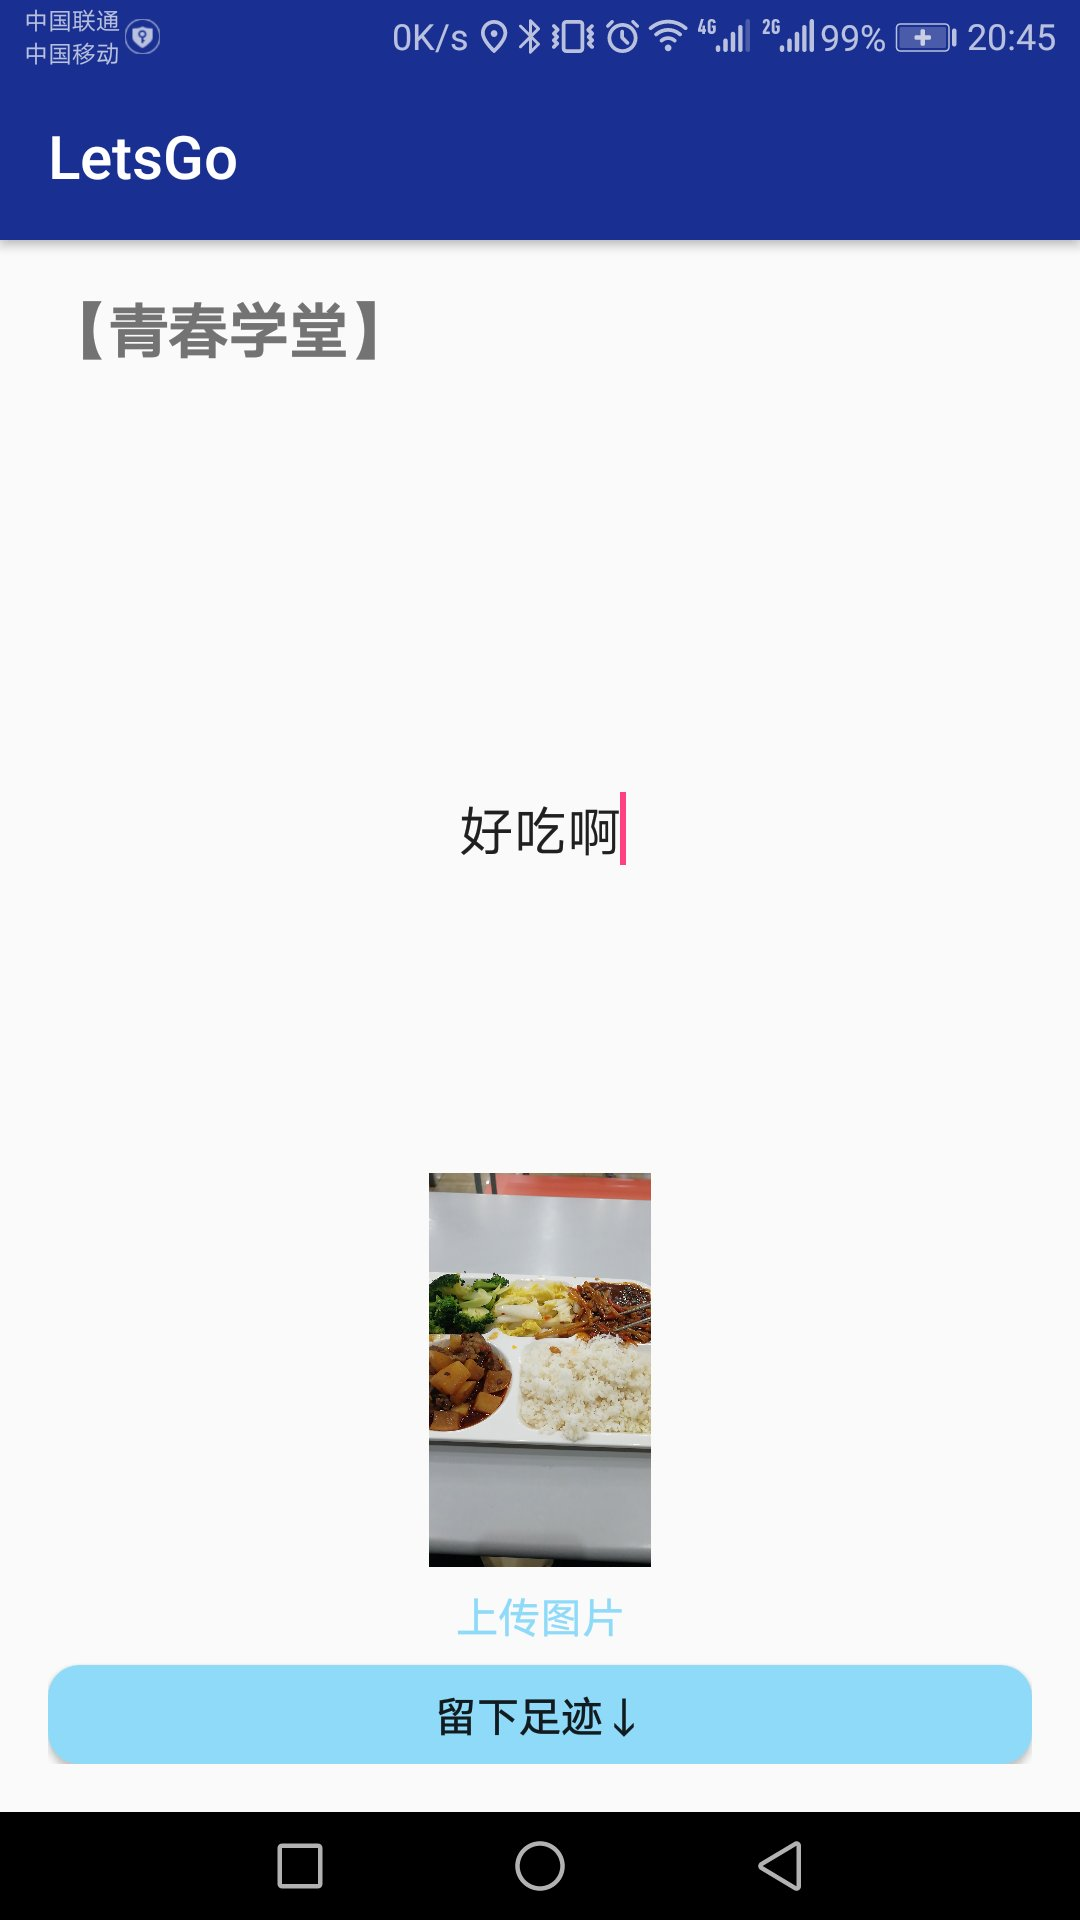
\includegraphics[width=\textwidth]{images/demo_post.jpeg}
    \caption{留下足迹}
\end{minipage}
\begin{minipage}[t]{0.33\textwidth}
    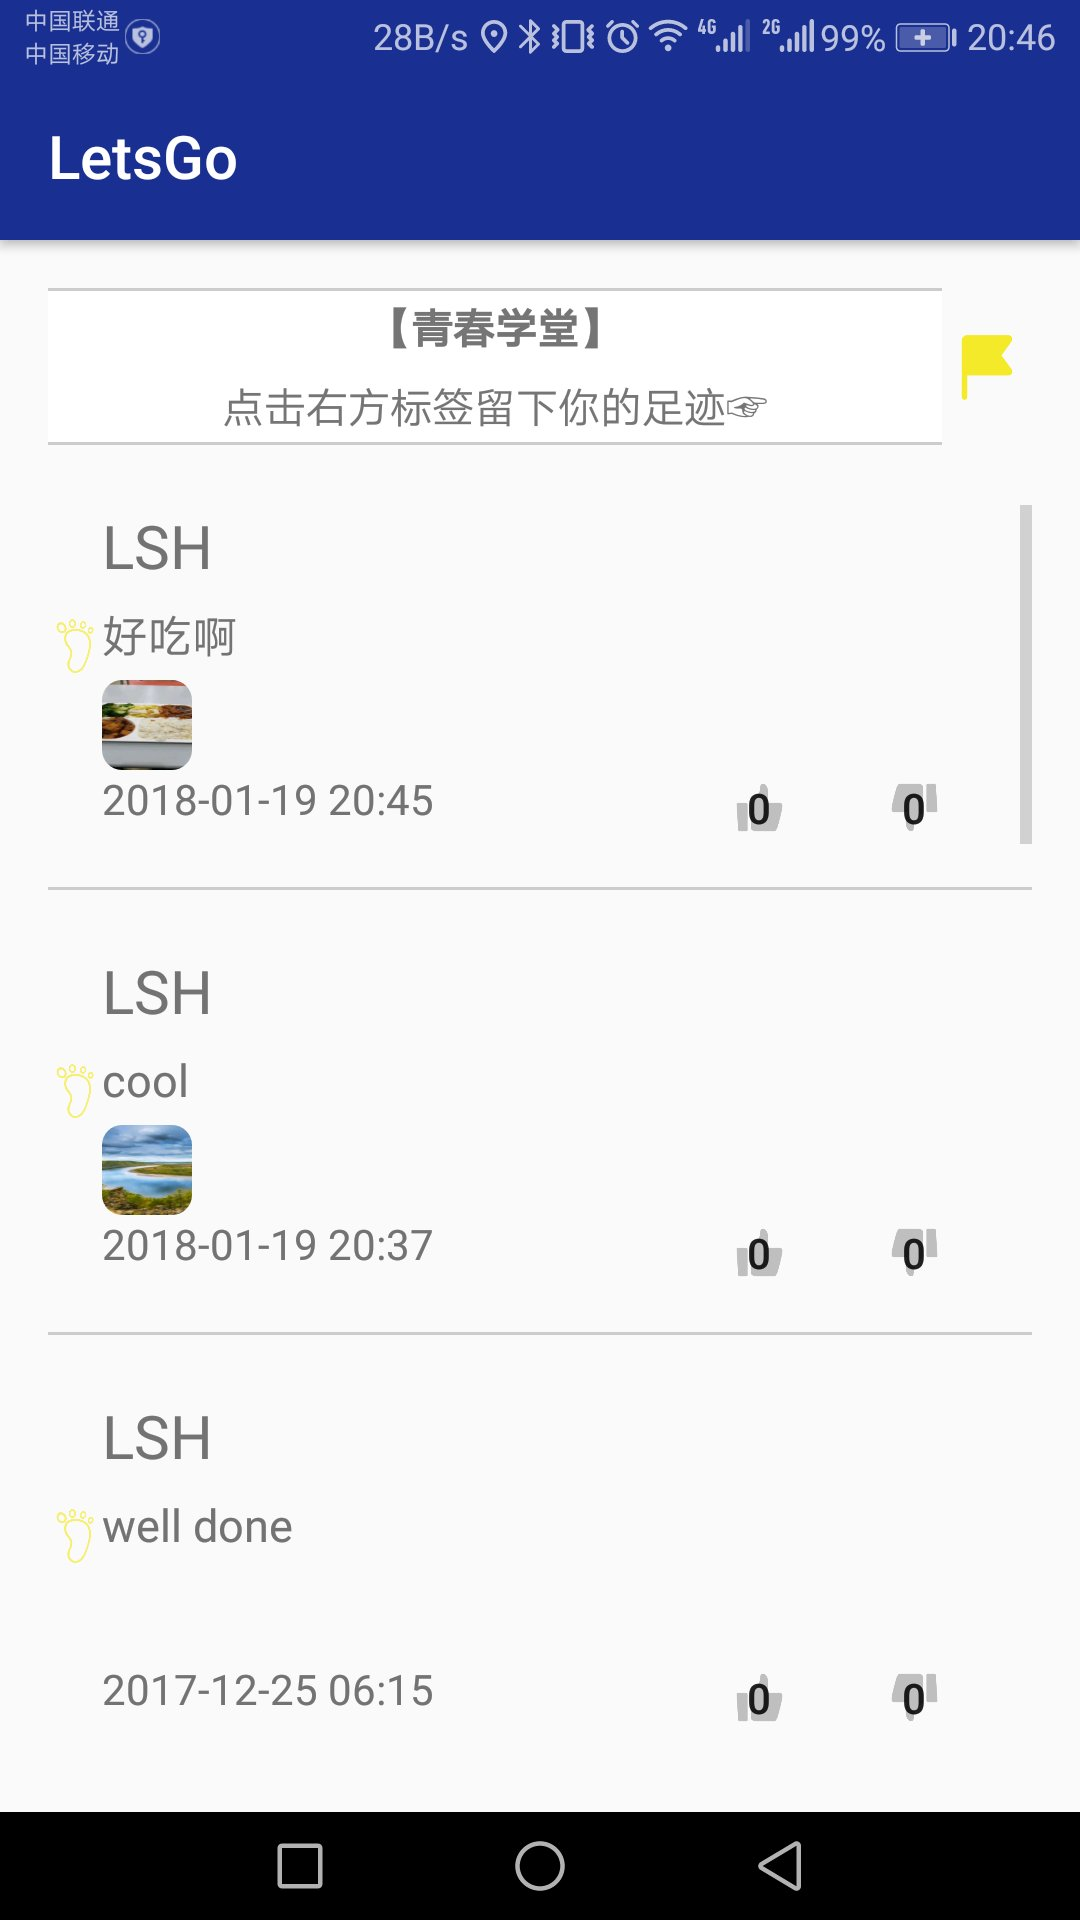
\includegraphics[width=\textwidth]{images/demo_browse.jpeg}
    \caption{浏览某一POI他人足迹}
\end{minipage}
\end{figure}

\begin{figure}[H]
\begin{minipage}[t]{0.33\textwidth}
    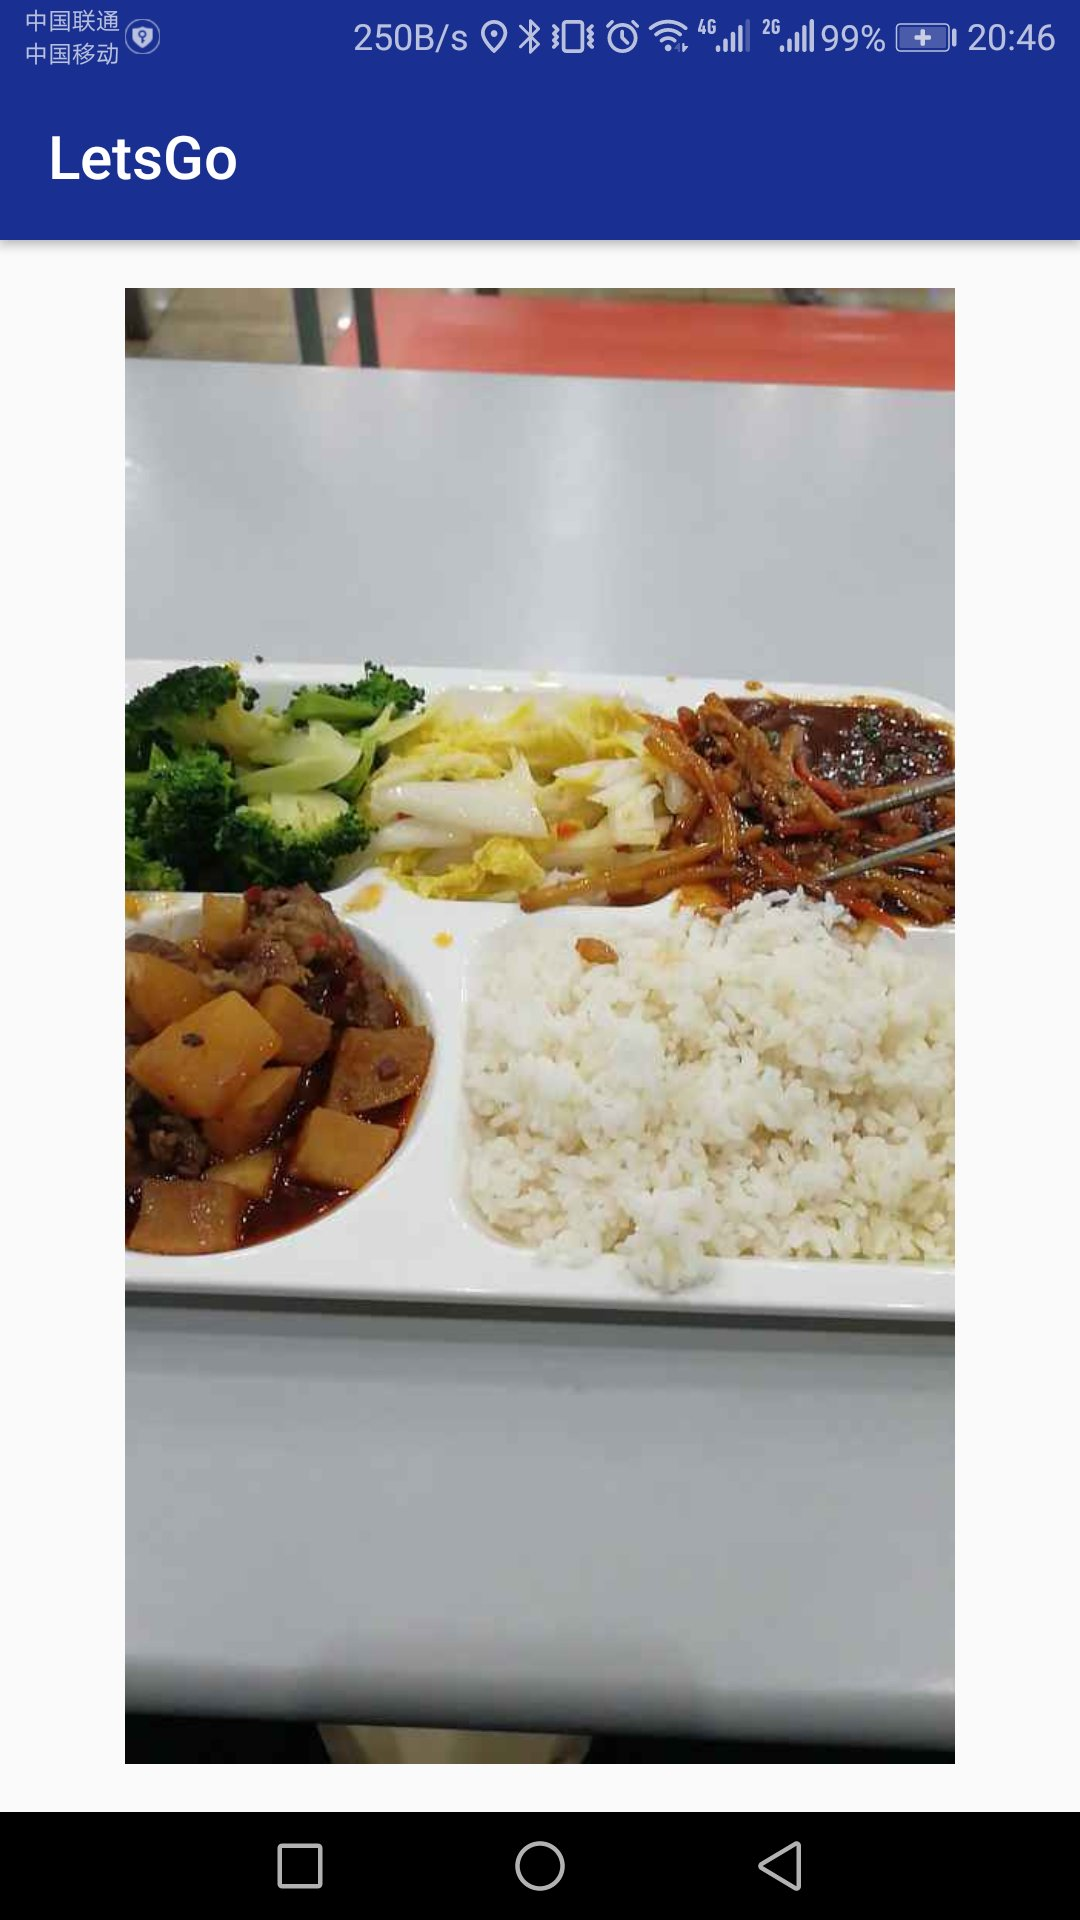
\includegraphics[width=\textwidth]{images/demo_picture.jpeg}
    \caption{放大查看图片}
\end{minipage}
\begin{minipage}[t]{0.33\textwidth}
    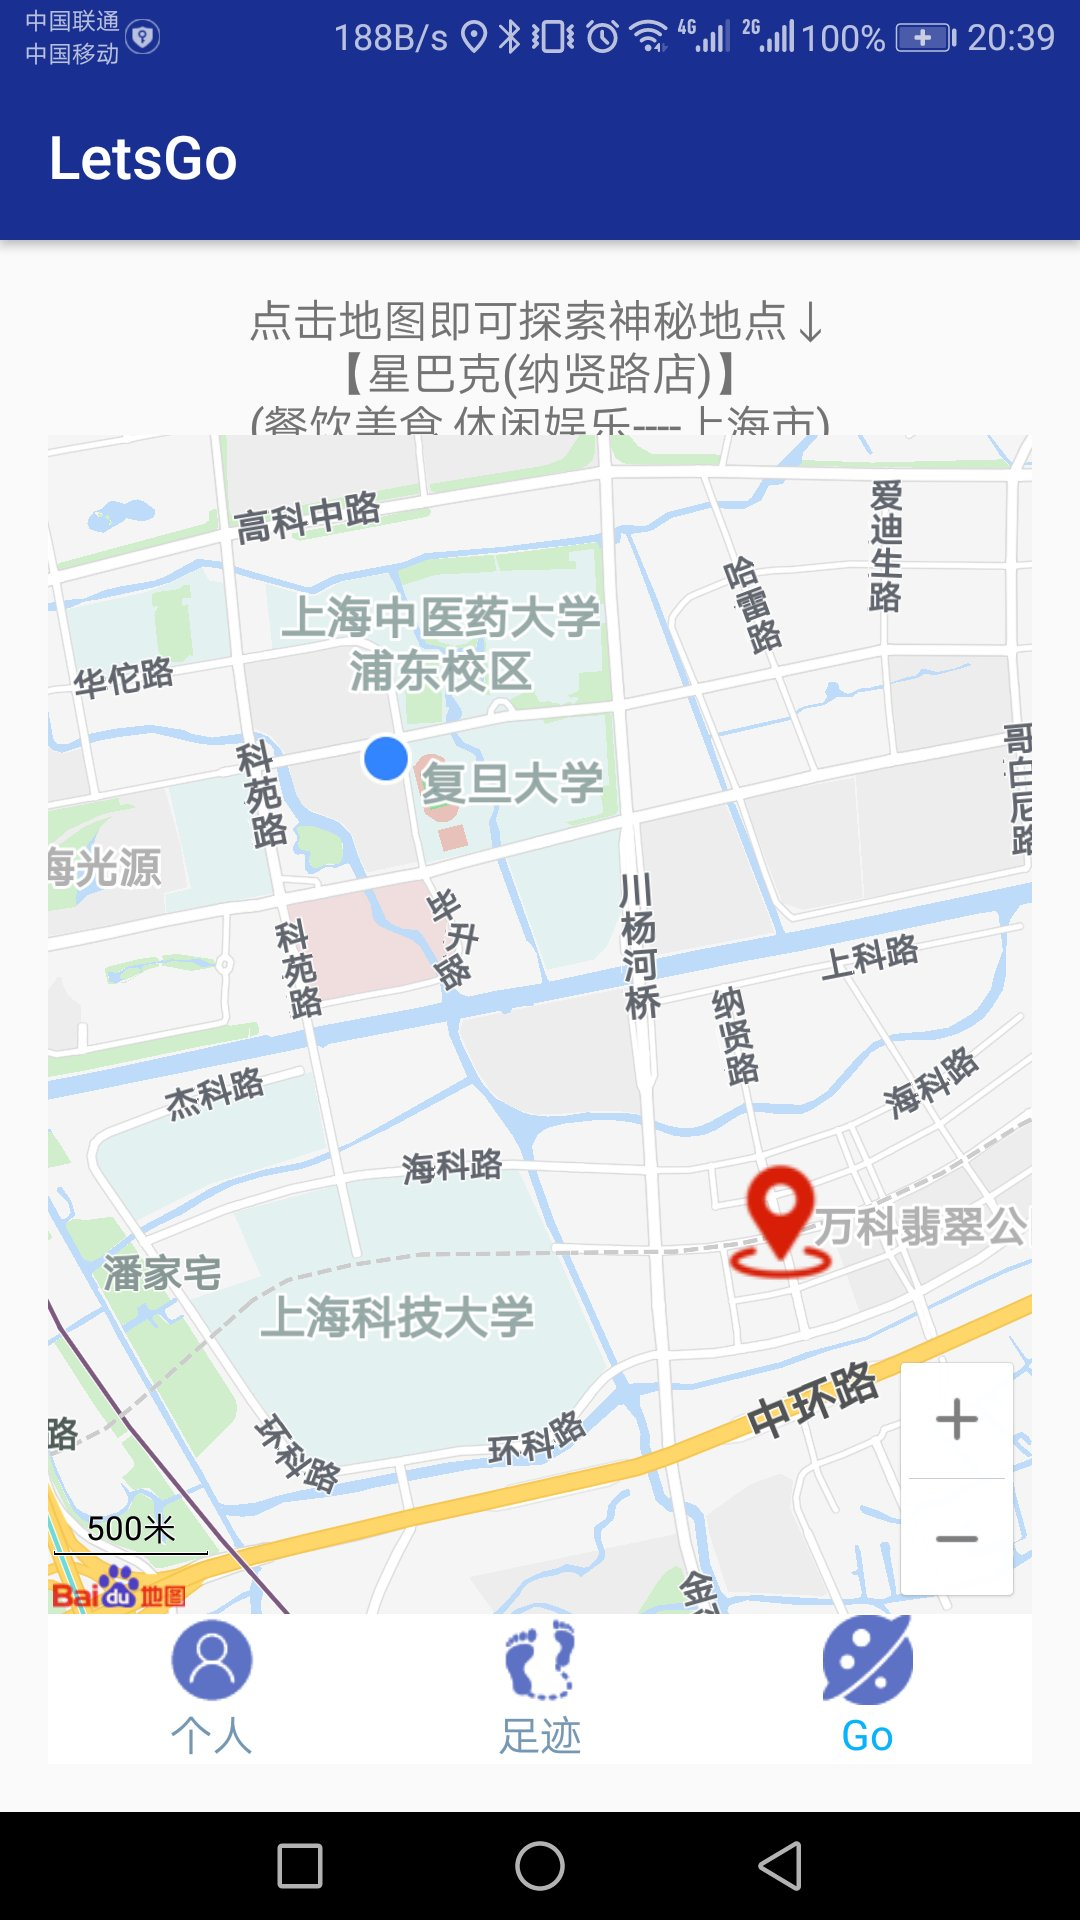
\includegraphics[width=\textwidth]{images/demo_recommend.jpeg}
    \caption{地点推荐}
\end{minipage}
\end{figure}

\section{分工}
Let's Go项目由赵浯旭(15307130231)和林士翰(15307130120)合作完成,赵浯旭负责了全部的客户端开发,林士翰负责了全部的服务器搭建和开发。
项目报告由两人共同编写。
两人的贡献比例为50\%:50\%。

\end{document}

